% \documentclass[oneside]{report}
\documentclass[oneside,final,14pt,a4paper]{extreport}
% \documentclass[journal,onecolumn,a4paper,12pt]{IEEEtran}
\usepackage[T2A]{fontenc}


\usepackage{vmargin}
\setpapersize{A4}
\setmarginsrb{2.5cm}{2cm}{2cm}{2cm}{0pt}{10mm}{0pt}{13mm}
\usepackage{setspace}
\sloppy
\setstretch{1.5}
\usepackage{indentfirst}
\parindent=1.25cm

%%%%% ADDED TO SUPPORT TT BOLD FACES %%%%
\DeclareFontShape{OT1}{cmtt}{bx}{n}{<5><6><7><8><9><10><10.95><12><14.4><17.28><20.74><24.88>cmttb10}{}
\renewcommand{\ttdefault}{pcr}
%%%%% END %%%%%%%%%%%%%%%%%%%%%%%%%%%%%%% 
\usepackage{atbegshi,picture}
\AtBeginShipout{\AtBeginShipoutUpperLeft{%
  \put(\dimexpr\paperwidth-1cm\relax,-1.5cm){\makebox[0pt][r]{
\includegraphics[width=3cm]{figs/inno}}}%
}}


\usepackage[english]{babel}
\usepackage[backend=biber,style=ieee,autocite=inline]{biblatex}
\bibliography{ref.bib}
\DefineBibliographyStrings{english}{%
  bibliography = {References},}
\usepackage{blindtext}
\usepackage{pdfpages}
\newenvironment{bottompar}{\par\vspace*{\fill}}{\clearpage}
\usepackage{amsmath,amsfonts}

\usepackage{amsthm}
\newtheorem{theorem}{Theorem}
\newtheorem{corollary}{Corollary}
\newtheorem{lemma}{Lemma}
\newtheorem{proposition}{Proposition}
\theoremstyle{definition}
\newtheorem{definition}{Definition}
\theoremstyle{remark}
\newtheorem*{remark}{Remark}
\theoremstyle{remark}
\newtheorem*{example}{Example}



\usepackage{float}
\usepackage{graphicx}
\graphicspath{{figs/}} %path to images
\usepackage{array}
\usepackage{multirow,array}
\usepackage{caption}
\usepackage{subcaption}
\usepackage{hyperref}
\usepackage{paralist}
\usepackage{listings}
\usepackage{zed-csp}
\usepackage{fancyhdr}
\usepackage{csquotes}
\usepackage{color}

\usepackage{upgreek} 
\usepackage{bm}
\usepackage{hyperref}
\usepackage{setspace}
\usepackage{booktabs}
\usepackage{multirow}
\usepackage{longtable}
\usepackage[font=singlespacing, labelfont=bf]{caption}
\counterwithout{table}{chapter}
\renewcommand{\thetable}{\Roman{table}}
%Hints
\newcommand\pic[1]{(Fig. \ref{#1})} %Ref on figure
\newcommand\tab[1]{(Tab. \ref{#1})} %Ref on table


\usepackage{enumitem}
\newlist{inlinelist}{enumerate*}{1}
\setlist*[inlinelist,1]{%
  label=(\arabic*),
}



\pagestyle{fancyplain}

% remember section title
\renewcommand{\chaptermark}[1]%
	{\markboth{\chaptername~\thechapter~--~#1}{}}

% subsection number and title
\renewcommand{\sectionmark}[1]%
	{\markright{\thesection\ #1}}

\rhead[\fancyplain{}{\bf\leftmark}]%
      {\fancyplain{}{\bf\thepage}}
\lhead[\fancyplain{}{\bf\thepage}]%
      {\fancyplain{}{\bf\rightmark}}
\cfoot{} %bfseries


\newcommand{\dedication}[1]
   {\thispagestyle{empty}
     
   \begin{flushleft}\raggedleft #1\end{flushleft}
}

% Table captions to support IEEE style
\captionsetup[table]{justification=centering, labelsep=newline}
\captionsetup[figure]{labelfont={bf},name={Fig.},labelsep=period}

\begin{document}

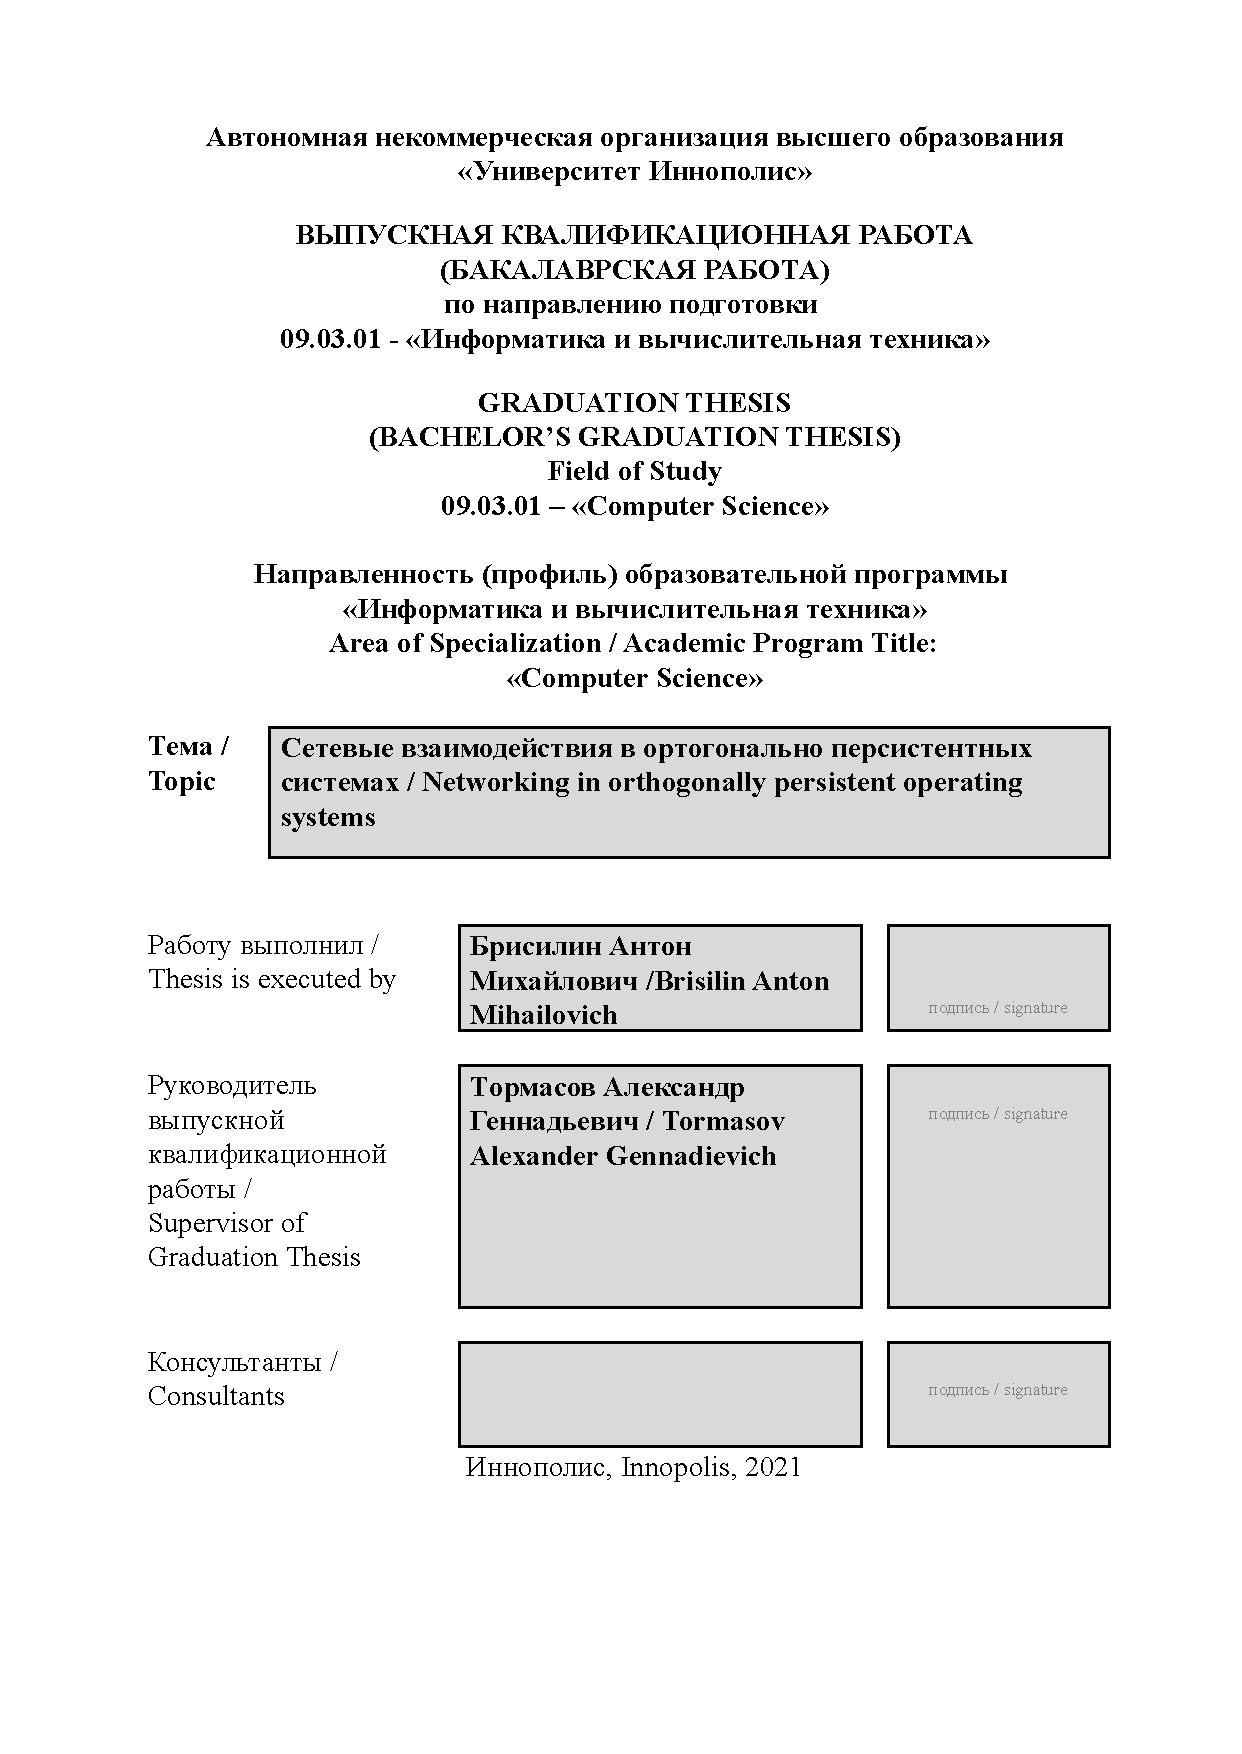
\includepdf[pages={-},offset=2.5cm -2cm]{title.pdf}
\tableofcontents
\listoftables
\listoffigures


\newpage
% \begin{abstract}
abstract \ldots
\end{abstract}
% Depend on above part
\setcounter{page}{7}
\chapter{Introduction}

\section{Background}
\label{sec:intro-bg}

Today, almost any enterprise application operates on data. A part of these data
often should be \textit{persistent}, that is, it should outlive the process
that created it. In this definition \textit{a process} is not an operating
system process, but instead a process is an abstract operation that creates
data. 

The division between persistent and non-persistent data is not dichotomic.
Several degrees of persistence exist -- from temporary values during expression
evaluations to long-stored records in a database. For example, when a customer
uses a bank card to purchase goods, the process is the withdrawal of money from
the customer's bank account. This process creates a record about the withdrawal
that can be seen later in a bank app. In case of expression evaluation, the
process is an execution of a CPU instruction. This process creates data:
instruction result that is stored in CPU register.

This range of data persistence closely resembles the memory hierarchy of modern
computers. Such similarity is for a reason: more persistent data are stored in
upper levels of memory. These memory levels are often energy-independent and
slower than lower ones. The presence of the memory hierarchy brings the need
for moving portions of data to lower memory levels when a program needs to
access a certain portion of data. On the other hand, the limited size of low
memory levels forces programmers to move data that is no longer needed to the
higher levels to free space for new data.

Modern operating systems and programming languages manage moving data between
the main memory and registers automatically, without the intervention from
application developers. However, when an application needs to access data from
a secondary storage, it should read and load data to the main memory by itself.
Writing a boilerplate program code for loading and saving data from and to
secondary storage adds more complexity to programs. Thus, it is a burden for
developers of those applications.

To remedy this management of moving data between memory layers, Atkinson and
Morrison \cite{atkinson1995orthogonally} propose to use persistent support
systems. These systems are a software for automatic management of physical
memory layers. The systems provide its users with a sandbox to run programs
where all data virtually have the same persistence.

\section{Phantom OS}
\label{sec:int:phantom}

The idea of persistent support systems was developed later with changing focus
to operating systems
\cite{landau1992checkpoint,dearle1994grasshopper,atkinson2000review}. These
systems have a notable property -- all data have the same persistence, and
their degree of persistence is high enough to outlive restarts of a system.
This means that the state of running programs is the same before and after
restarts.

The most modern persistent OS up to date is Phantom OS. This operating system
consists of a stateless kernel and a Phantom Virtual Machine (PVM). PVM hosts
processes, which execution states persist across restarts of the host machine.
Persistence is achieved with periodic snapshotting. In the context of Phantom
OS, a snapshot is a memory dump of the PVM memory space. The system uses the
latest snapshot as a recovery point on booting.

Even though Phantom OS is a working persistent support system, there is still a
room for improvement. Currently, Phantom OS does not restore the state of the
Transmission Control Protocol (TCP) stack. The operating system only handles
sockets in the LISTEN state. If a socket was in this state when the snapshot
was taken, the system will reopen it on boot, bind to the same address and
start listening on it. Sockets in other states will become invalid. Any
attempt to use these sockets will result in an error. The application that
tries to use such a socket will receive this error and will be responsible for
its handling. Usually, that handling implies reestablishing a connection with a
remote peer and restarting data transmission from the very beginning.

Because of the presence of these errors, existence in a persistent environment
is not completely transparent for Phantom OS applications. Moreover, the common
way of handling these errors, which was described above, results in inefficient
network use, especially when power is off for a short period of time.

\section{Problem statement}

Recently, a group of researchers from Innopolis University started porting
Phantom OS to the Genode OS framework. The PVM in this port is implemented as a
userspace Genode process, and all the Phantom kernel syscalls are implemented
as functions provided by the Genode layer of the port. In particular, the
network stack was implemented in the Genode as a Virtual File System (VFS)
plugin. Due to this fact and the flexibility of the Genode VFS, changing
implementation of the networking stack became easier in comparison to Phantom
OS before this port. 

The functionality of restoration of sockets state was not in the scope of this
port. Thus, even the inherent Phantom OS ability to restore listening sockets
was lost in the porting process. My hypothesis is that it is possible to
develop an enhancement to the networking stack of Phantom OS port. This
enhancement should reside entirely in the Genode part. The enhancement should
provide client applications with an abstraction of a persistent socket, i.e.
socket that can be used after any number of restarts of a host machine. To
simplify the problem I will implement the mechanism working only for
short-duration shutdowns that get unnoticed by the remote side. However, in
the theoretical part of this thesis I will consider cooperative mechanisms
that could allow handling longer shutdowns.

The original document describing TCP \cite{john1981transmission} suggests using
a single Finite State Machine (FSM) per socket to implement the protocol. Most
implementations of the protocol, including the one used in Phantom-over-Genode
(PoG) port, use this FSM technique. The theoretical challenge behind an
implementation of the enhancement described above is the integration of an
external state machine into the Phantom persistence model. In this context,
“external” means that the code of the state machine is not running as managed
code inside PVM. Thus, the first aim of this paper is to develop a methodology
for integrating such state machines into Phantom OS. 

The second aim of this paper is to enhance PoG TCP stack to achieve two goals.
The first goal is to reduce the number of errors that should be handled by
applications supervised by the PVM. This means that as many errors as possible
should be either prevented or handled at the Genode layer of the OS. The second
goal is to make the network utilization more efficient. This means avoiding
extra TCP transmissions, if they are not necessary.

The rest of this thesis is structured as follows: Chapter \ref{chap:lr}
contains a detailed description of the persistence concept, brief overview of 
relevant details of TCP, general description of Phantom OS, the Genode OS
framework  and a review of related work in creation of persistent networking
stacks. Chapter \ref{chap:meth} establishes requirements for the implemented
software and discusses approaches that in theory could be used to implement it.
Chapter \ref{chap:impl} discusses relevant implementation details of the PoG
port, approaches that were tried during the implementation, and reasons
why some of them were discarded in favor of the others. Chapter \ref{chap:eval}
contains a description of the achieved results, description of experiments to
evaluate them and future directions.  Chapter \ref{chap:conc} contains a brief
summary of this paper.


\chapter{Literature Review}
\label{chap:lr}
\chaptermark{Second Chapter Heading}

This chapter begins with an overview of the concept of persistence in general
and orthogonal persistence in particular in Section \ref{sec:lr:persistence}.
The Section \ref{sec:lr:networking} describes what special networking needs
do persistent systems have and then presents an overview of the TCP protocol,
which will be useful in next chapters. The last section of this chapter
briefly describes Phantom OS, Genode OS framework and the current state of
porting the former to the latter.

\section{Persistence}
\label{sec:lr:persistence}
\subsection{Persistence definitions}

The concept of \textit{data persistence} was informally introduced in Section
\ref{sec:intro-bg}. The formal definition of this concept is presented below.
\begin{definition}
The lifetime of a data is a time extent over which it can be used. This
lifetime is commonly called \textit{persistence} \cite{atkinson1983ps}. 
\end{definition}

Atkinson \textit{et al.} \cite{atkinson1995orthogonally,atkinson1983ps} give a
classification of application data by their persistence. This classification is
presented in Table \ref{tab:data_lifetimes}. As it was said earlier, the
support of levels 1-4 is usually provided by an operating system and a
programming language. This is due to the fact that these data are stored at the
main memory or lower memory levels. On the other hand, to have data with
persistence of levels 5-7, applications designers should rely on some external
component, such as database or file system. 

\begin{longtable}{cl}
\caption[Classification of data based on their lifetime]{Classification of data
based on their lifetime} 
\label{tab:data_lifetimes} \\
\hline
1. & Intermediate results in expression evaluation \\
2. & Local variables inside functions and code blocks \\
3. & Global variables and heap items \\
4. & Data that exists throughout a whole execution of a program \\
5. & Data that lasts for several executions of program \\
6. & Data that lasts for as long as a program is being used \\
7. & Data that outlives a program \\
\hline
\end{longtable}

\subsection{Orthogonal persistence}
\label{sec:LR:orth-persistence}

As was stated in section \ref{sec:intro-bg} using inherent programming
languages mechanisms and external mechanisms to access data interchangeably is
a burden for programmers. Presence of different data formats in each of these
storages makes this burden even heavier. As mentioned earlier, in response to
this problem, \cite{atkinson1995orthogonally} proposes to use persistent
support systems, which act as a mediator between supervised applications and
a transient environment. Atkinson \textit{et al.} also summarize design
requirements for such systems, which they call \textit{Principles of Orthogonal
Persistence}. The authors define the following requirements for an orthogonally
persistent support system: 

\begin{enumerate}
    \item The Principle of Persistence Independence. 
    
    Whether a program manipulates data that outlive it or not, the ways to use
    these data should be the same. There should be no significant difference in
    program syntax in either case.

    \item The Principle of Data Type Orthogonality. 
    
    Any part of data should be allowed to have any level of persistence, 
    irrespective of their type. There should be no special cases where objects
    of some type can not be persistent or transient.
    
    \item  The Principle of Persistence Identification. 
    
    The choice of how to identify which objects are persistent and how to
    provide persistence to them is not related to the universe of discourse of
    the system. The mechanism for identifying persistent objects should not also
    be related to the type system.

\end{enumerate}

A system that treats data according to these three principles is said to be
\textit{orthogonally persistent}. Two popular approaches exist to build such a
system. The first one is to integrate interactions with databases or file
systems into existing programming languages. In this case a program syntax to
access data stored in the memory should look the same as access to data in a
database. But semantics behind this syntax can vary. This idea is quite similar
to the work of modern Object-Relational Mapping (ORM) libraries
\cite{аннин2018краткий,copeland2008essential}. However, this approach is not
really orthogonally persistent since most ORM libraries put certain limitations
to what can be saved to the database. It also is sometimes problematic because a
different meaning behind seemingly similar fragments of code confuses
programmers.

The second approach is to build so-called \textit{persistent worlds} 
\cite{atkinson1995orthogonally}. These worlds usually have the form of an
operating system or a virtual machine. Applications residing in persistent
worlds are usually written with managed code. From now on I will use the term
\textit{persistent applications} for resident applications of persistent
worlds.

The fact that persistent applications are generally written with managed code
enables a system to automatically manage states of the applications so that they
have a consistent behavior across restarts. The examples of such systems are
KeyKOS \cite{bomberger1992keykos}, Grasshopper OS \cite{dearle1994grasshopper},
and Phantom OS. 

Creation of persistent support systems that work with nonvolatile memory (NVM)
as a main memory is an emerging research direction in the field of persistent
support systems. This approach seems to be more convenient for implementation
of orthogonally persistent systems, but it still has unsolved problems. The two
examples of such problems are the problem of dealing with changed states of
peripheral devices after restarts \cite{berthou2018peripheral}, and logical
problems with code execution \cite{ransford2014nonvolatile}. That is why the
creation of such systems is not a trivial question. 

\section{Networking in persistent systems}
\label{sec:lr:networking}

The nature of persistent applications implies that their execution can be
interrupted and then resumed after some time, when a host machine reboots. This
creates a challenge when an application is designed to communicate with remote
peers with a stateful network protocol. The challenge is to synchronize
states of the communicating peers: while a local system is offline a remote peer
can change a state of the connection indefinitely. Moreover, some persistent
support systems, like Phantom OS, use snapshotting to create an illusion of
uninterrupted execution. In case of such systems, the challenge is even more
problematic, because a persistent peer can "forget" that it had sent or received
some data. This happens if a record about data transfer was not embedded in a
snapshot, for example due to an unexpected power loss.

\subsection{Transmission control protocol}

The most popular transport layer protocol -- TCP -- is designed to provide a 
reliable packet delivery service. The reliability is achieved with periodic
retransmissions and acknowledgements. TCP packets are called segments. Each TCP
segment is equipped with two numbers - SEQ and ACK. SEQ, or \textit{sequence
number} is a number of payload bytes sent by the sender of the segment before
the current one. ACK, or \textit{acknowledgement number} stands for number of
payload bytes the sender received. To enhance the security and error tolerance
of the protocol initial SEQs are chosen randomly at the connection
establishment time. To enable error-detection TCP segments carry checksum that
comprises contents of the segment and so-called pseudo IP header
\cite{tcp_ip_illustrated_vol2}. The checksum can be updated incrementally,
without recomputing it for a whole packet \cite{rfc1624}.

When a host receives a TCP segment, the host's TCP checks the segment's SEQ
number. If SEQ is equal to $N$ and the last previously acknowledged byte had
number $N-1$ the segment is accepted and payload passed to the user of the TCP.
After the payload is queued to be delivered to the user, the receiving TCP
sends an acknowledgement segment with ACK equal to $N$.

TCP is a connection-oriented protocol. Before any data transmission happens,
communicating peers need to establish connection to negotiate transmissions
parameters. These parameters include exchange of initial SEQs. The connections
are established with a three-way handshake, that is, exchanging of three
segments - two from client to server, and one in the opposite direction.

TCP uses retransmissions and acknowledgements as follows. When a remote peer
does not acknowledge a packet TCP prescribes to retransmit it. The maximum
number of retransmissions is not stated in the original TCP specification
\cite{john1981transmission}.  However, the specification received updates
later, which prescribe to retransmit packets with exponentially increasing
delay \cite{rfc6298} until the timeout of at least 100 seconds \cite{rfc1122}.
This means that some TCP implementations will close a connection if their
peer appears to be down for more than 100 seconds.

The closing of connection when a host is temporarily offline is a good example
of a problem with traditional stateful protocols. The example highlights that
persistent support systems should restore the state of network connections in
the restoration phase when the execution was interrupted by a power loss.
Several approaches were proposed to hide closing of connections from user
applications.  The first approach, proposed by Ekwall, Urb{\'a}n and Schiper
\cite{ekwall2002robust}, is to create a session layer protocol that will behave
similar to the original TCP specification with respect to timeouts. That is,
the protocol will retransmit packets infinitely reopening underlying TCP
connections as they get closed.

The second approach was proposed by Zhang and Dao \cite{zhang1995persistent}.
This article, as well as the previous one, proposes to use a session-layer
protocol to create an abstraction of persistent connections, i.e. connections
that outlive execution of a one peer. The authors propose to use a centralized
notification service to transfer control messages. When this service detects
that a process goes down the service notifies all peers communicating with the
process. These processes switch their ends of connection to passive mode. In
this mode blocking read operations are getting blocked, and writes are buffered.
When the down process resumes its execution it registers in the notification
service. The former peers of the process receive this notification and try to
establish a connection to the continuation of the process. However, this
approach can lead to loss of data that were in flight when a process comes down.

Creation of a session-layer protocol on top of TCP is not the only way to
implement persistent connections. Zandy \textit{et al.} in \cite{rocks_racks}
propose a mechanism that hides disappearance of a remote peer from applications
that use TCP. The mechanism named \textit{rock} employs heartbeat probes via a
separate UDP control socket to detect if a remote peer is gone. When a process
detects loss of connection with a remote peer the process repeatedly tries to
reconnect to its peer by the last known physical address. If loss of a peer was
caused by network error, this will eventually succeed. Otherwise, the
reconnection attempt will be timed out. However, the rocks mechanism provide
a large timeout and it can be changed in per-connection basis, unlike TCP. 

To avoid loss of in-flight data while a process restarts a rock keeps a buffer
sized as a sum of local host send buffer size and peer host receive buffer
size. The buffer is used in a similar way as the send buffer is used in TCP:
the packets in the buffer are used to perform retransmissions.

\section{Phantom OS and Genode OS framework}
\subsection{Phantom OS}

Phantom OS is a general-purpose operating system, developed in 2009-2011. The
operating system consists of a stateless kernel and virtual machine, which
executes userspace applications. Phantom OS applications are written in Phantom
programming language. The execution of managed code is persistent, which makes
Phantom OS a persistent support system. As was said earlier, persistence for the
managed code is achieved using snapshotting. Phantom is an experimental system,
in a sense that it is developed as a proof-of-concept and is not ready for
production use.

Phantom OS currently supports only i386 ISA and it has all drivers embedded 
inside a kernel. It is problematic, because to support wide range of hardware
OS needs drivers, which is often delivered by third-party developers. But in
case when drivers are embedded in kernel an error in driver can crash the whole
system. Implementation of drivers as parts of kernel also complicate
development and delivery of the drivers.

These are two reasons why it is desirable to replace Phantom kernel with a
microkernel. The port of Phantom OS to the Genode OS framework is being
developed right now. It is implemented as a Genode component running the PVM.
This means that network capabilities are provided by the Genode level of the
PoG port.  That is why I will concentrate my attention on development of a
network stack working in Genode.

\subsection{Genode OS framework} 
The Genode OS Framework \cite{genode_foundations} is a toolkit for creating 
operating systems. It provides a possibility to build a microkernel operating
system from set of existing components. Genode also provides an API to
integrate various microkernels into it.

For now the supported kernels include Linux kernel, nova microhypervisor and
several kernels from the L4 kernel family. Supported kernels from the last
family include L4ka::Pistachio, Fiasco.OC, formally verified seL4 microkernel,
and L4/Fiasco.  The framework also supports execution on bare hardware on ARM
and x86-64 ISA.

The Genode itself provides mechanisms for threading and synchronisation,
inter-process communication (IPC), virtual memory, pluggable device drivers,
sandboxing, and VFS. Processes in Genode are called \textit{components}. Genode
components usually belong to one of the five categories: device drivers,
resource multiplexers, protocol stacks, applications and runtime environments
\cite{genode_foundations}. Genode's VFS with possibility of adding custom
plugins to it. For instance, the ram-fs plugin can expose a part of process
memory as a file. This is particularly convenient when one uses libc that has
an API that is mostly file-oriented. TCP/IP stacks are also implemented as VFS
plugins that represent each socket as a set of files. VFS plugins are merely
shared libraries that are loaded by VFS at runtime. Genode applications are not
linked with VFS plugins.

Genode's IPC mostly consists of blocking remote procedure calls (RPC). To use
an RPC object provided by a server component, a client component should have a
\textit{capability} to call it. A capability is a special reference to an RPC
object which is backed by the kernel. Possession of capability is enough to use
an object that it references to. Capabilities are typed with the RPC interface
they provide. Genode components have capability quotas - maximum number of
capabilities they can own.

Genode TCP stacks use the Network interface card (Nic) RPC interface as an
input and output. That is, TCP stacks submit and receive packets via these
interfaces. The Nic interface is implemented by a regular userspace component
and therefore its implementation can be changed on a per-component basis.

Genode VFS plugins and Genode components in general are not persistent. TCP
stacks lose their state after a power loss. Therefore, I need to implement
saving and restoring of state of a TCP stack before it can be used by PVM.

\chapter{Methodology}
\label{chap:met}

This chapter starts with the analysis of requirements for implemented software.
After that, the implementation is discussed in more detail in the dedicated
section.

\section {Requirements analysis}

As previous chapters of this paper suggest, the goal of this paper is to create
an implementation of a TCP/IP stack suitable for a persistent system. In
particular, I use a port of Phantom OS to Genode OS framework as a target
platform.

This section contains a list of requirements that a developer of such a stack
should take into account when implementing their own port.

\subsection {Transparent peer disappearance}
One of the fields in which persistent systems are actively applied is IoT. In an
intermittently powered environment, a system that can efficiently restore its
state is preferable to a system that experiences a booting process that consumes 
a lot of energy.

In such cases, hosts can experience long downtimes. Standard TCP implementations
are not applicable here because they perform retransmission of packets for only
a limited amount of time, and then close connection.

To make the development of stable persistent applications easier a temporary 
shutdown should be transparent for the client app. That means that the network 
connections state should be the same when the powered-off host restarts.
To achieve that persistent TCP implementation should either (1) backup and
restore connections state or (2) make the disappearance of the remote peer
invisible for application on the other end of the connection.

\subsection {Rollbacks}

The technique used in Phantom OS to provide persistence is memory snapshots of 
PVM memory space. They are taken in a live mode so that processes inside the VM
continue to run. Then, when power is back on, the latest snapshot is restored by
copying it to the main memory. The part of Phantom that is outside of VM is
assumed to be stateless in the usual case, which is not the case in Genode port.
That is why snapshotting and restoring of Genode part of the system is done with
callbacks, which accept and provide blobs of data to be saved in persistent 
memory. 

In the case of the intermittently powered Phantom system, this can cause
trouble, when clients actively use networking. While the system performs a
snapshot, the TCP stack can still proceed with receiving data. In this case,
TCP on receiving side will acknowledge packets, as protocol prescribes.
The issue is that acknowledged packets are getting deleted from the
retransmission queue, and therefore not present at the sending site. However,
they are not present in the snapshot on the receiver's side. In this case, after
the snapshot is used to restore the state of the receiver, the receiver will
request the packet (with duplicated ACK) that the sender is unable to 
retransmit. In this case, the sender's TCP will respond with RST and then close
the connection.

Three solutions exist that may solve the problem above. One is to forbid
sending acknowledgment packets if a received packet is not included in any
snapshot. However, this will either dramatically increase the number of
retransmissions in a network, which will result in reduced network performance
or it will require doing snapshots very often. In such a case snapshot should
be performed each 50ms. With a snapshot duration of around 10 seconds, this is
not acceptable.  

The other solution is to keep a buffer in a persistent memory that will store
all packets that a user of TCP had not consumed yet. In this case, persistent
memory can be a regular file or memory space that will fall into a snapshot for
sure.

The third approach is to have a dedicated broker inside a network that will
function similarly to the buffer in the second case. The broker can save all
acknowledged packets in a network, and flush its queue when it detects that
receiving host has done a snapshot. ICMP messages or some similar mechanism
will be useful to notify the broker about the end of the snapshot process.

\subsection {Compatibility with existing protocols}

The third design goal is not directly related to providing persistent I/O
abstraction to the clients of a network stack. Since snapshotting is a very
popular technique for implementing persistent systems, and Genode is actively
used to develop various operating systems, it is probable that some other
developers might want to use persistent TCP in their software.

That means that result of this work should be a standalone application that
works without Phantom and is flexible enough to support all use cases that may
arise. Fortunately, Genode's component-based architecture helps greatly with
it.

Another thing that should be addressed in the design of the API of the system,
is easy migration from non-persistent TCP stacks already available in Genode,
namely lwip and lxip. To do this I intend to design API very similar to regular
sockets or even exactly the same, but with different call semantics. I also
plan to add a Virtual File System (VFS) plugin that will expose sockets as
regular files because this is the way how Genode developers suggest
integrating sockets into the Genode ecosystem since version 18.11. With such
implementation, even relinking of existing binary will be not needed. The only
thing user would need is to change the configuration of the init Genode
component.

\section{Implementation process}

I have chosen to implement a persistent TCP stack in form of a Genode component
that will serve as a plugin for a VFS. The users of the TCP stack should add
signal handlers to their components for signals of type SIG\_SNAP and
SIG\_RESTORE. When SIG\_SNAP is received, it is passed to the persistent TCP VFS
plugin which gathers data that should be saved into persistent memory and calls
filesystem service to save socket snapshot structure into persistent memory.

Symmetrically, when SIG\_RESTORE is received, the component will access the
previously saved file and read information about sockets state at the snapshot
moment.

The exact structure of the data needed for the connection restore process and
some conditions for successful persistence of sockets will be discussed in the
following sections of this chapter.
\include{chapters/chapter4-Implementation}
\chapter{Evaluation and Discussion}
\label{chap:eval}

This chapter begins with the brief description of achieved results. The second
section discusses of how the requirements formulated in section
\ref{sec:meth:req} were implemented in PTCP. Then the chapter discusses testing
scenarios created to test if the implemented mechanism works. After that the
results of tests are discussed. The end of the chapter contains future
directions in a field of network stack of PoG port.

\section{Results}
\label{sec:eval:res}

During this work I created a PTCP mechanism in form of Genode VFS plugin,
Genode Nic proxying component and a shared library. The mechanism can be used
to restore states of TCP sockets if execution of a program was interrupted by a
shutdown. In particular, this can be useful for Phantom OS port to Genode OS
framework. 

The current limitations of the PTCP mechanism is that it is only works with
TCP sockets in closed and listen states. However, this limitation is only due
to the lack of time. In principle, nothing blocks addition of code for handling
other states. With this limitation, however, PTCP is still useful with the PoG
port, because its capabilities are the same as ones of the Phantom OS kernel
TCP stack. The PoG port aims to replace the Phantom kernel with Genode
components. Hence, PTCP can be a suitable replacement for the TCP stack
previously implemented as a part of Phantom kernel. Furthermore, PTCP is easier
mantained, because it is independent and its codebase is quite small.

\section{Meeting the requirements}

\subsection{Transparency for client applications}

PTCP is not completely transparent for client applications. To use it, 
application should use a PTCP client library and add function call that will
initialize the library at component startup. This lack of transparency is a
result of compromise between problem of creation of persistent socket names and
unwillingness of modifying Genode libc. I do not want to modify libc because it
belongs to a trusted computing base. Any change in it should be done with
caution and should be verified. 

If an application does not need the persistent sockets functionality and
instead wants to use PTCP as a regular TCP stack then PTCP acts as any other
TCP stack available in Genode. That is, PTCP VFS plugin is added as a backing
plugin for socket directory and path to the directory is passed to libc.

\subsection{Robustness to rollbacks}

PTCP fails to properly process rollbacks. In case of unexpected shutdown
packets that were received by PTCP but were not delivered to applications will
be lost. However, the architecture including a proxying Nic component allows
PTCP to replay the packets that were in reception queue when a host machine
came down. However, in this case PTCP should somehow track what packets are 
in a send queue and this seems to be challenging.

\subsection{Usefullness}

The usefullness requirement was satisfied by PTCP. For now the developed
prototype already can serve as a replacement for Phantom OS TCP stack. I will
not stop on this requirement in detail, as it already was discussed in the
Section \ref{sec:eval:res}.

\subsection{Compatibility with the existing protocols}

This requirement, in essense was about using TCP or some other well-known
protocol. This requirement holds in PTCP. The TCP stack uses TCP protocol and
can be used by Genode components exactly as they use any other TCP stack.

\section{Testing scenarios}

I created two test cases that emulate behavior of a persistent system using 
PTCP. These cases are quite simplistic and only designed to check correctness
of work of the developed software.

The first testcase checks that TCP sockets in various states are restored
correctly. The program creates six TCP sockets. Two of these sockets remain in
the closed state. The two of them are bound to local ports to be later used in
listen() function. The rest two are bound to addresses and then their states
set to the listen state. All sockets are bound to the different ports.

After this initialization the test scenario remembers which socket has which
persistent descriptor. Then the scenario saves the mapping to persistent memory
and ensures that PTCP have made its snapshot. Then a restart is scheduled.
After the restart the test case loads mapping between sockets and descriptors.
At this point PTCP should have its state restored, because restoration takes
place before passing control to client application. After the mapping is loaded
the test case checks that each socket is in valid state. The checks consists of
moving each socket to listen state with Berkeley socket API and ensuring that
socket really listens by connecting to the machine from another machine in the
same subnet. If any socket returns any error in process of verification or 
initialization, the test case considered to be failed.

The second test case is designed to check that PTCP can correctly process
sending and receiving packets. This test case works similarly to the previous
one -- it also consists of initialization and verification phases separated by
a restart. The initialization part includes setup of a listening socket. When
the socket is open, a remote machine establishes connection to the PTCP client
application and expects to receive 100 packets with a certain payload. After
connection establishment the server machine sends packets. It performs snapshot
after each packet is sent. When it sends 50th packet, the server machine shuts
restarts. After the restart the test case on the server reads number of sent
packets and proceeds sending the payload starting from 51th packet. The point
of this test is to check the work of the Nic proxy mechanism. The fact that
the old server socket does not exists anymore should not be noticed by the
client process. Unfortunately, for now this test always fails because the proxy
was not implemented.

\section{Future directions}

PTCP only works with changing of state of only one machine. Therefore, the
state of a connection can be restored only when the socket at the remote site
exists. This limits a possible time when PTCP can restore sockets. In most
cases the time that a host can be down is around of 30 seconds. This is quite
small amount of time and. To make it larger PTCP should be a collaborative
mechanism. Communicating PTCPs may employ exchange control messages, as
proposed by \cite{rocks_racks}, for example by using a separate UDP socket or
ICMP messages.

Another issue that might be addressed is change of interface's IP address after
restart. Throughout this paper, I discussed PTCP mechanism under the assumption
that IP address does not changed. However, it is not always the case in the
real world. In case of change of IP address the remote peer will not be able
to consider newly created socket as a continuation of the previously existing
one. One can implement a proxying NAT-like server similar to the Nic proxy
discussed above. However, this server should live outside the persistent
machine and have static address.

% TODO restoring seqs is insecure
% TODO Fd_proxy can't create multiple sockets at same time


\chapter{Conclusion}
\label{chap:conc}

During this thesis I have described and implemented the PTCP mechanism for
providing an abstraction of persistent TCP sockets for the client applications.
The mechanism was initially intended to be used together with the port of
Phantom OS to Genode OS Framework. However, the mentioned port was not finished
before this work. That is why I narrowed my scope to implement software that
can be used with Genode only. I nevertheless believe that the PTCP can be
easily integrated to the upcoming PoG port. It is used in the same way as any
other Genode TCP stack with minor additions, therefore switching to it should
not be a problem.

However, there are still limitations in the current version of the PTCP. It
functionality can be improved to meet requirement for an ideal persistent TCP
stack, as described in the Chapter \ref{chap:meth}. It can include support for
client sockets in established state, as well as handling of longer shutdowns
with some sort of cooperation mechanism.


%% REFERENCES
\printbibliography[heading=bibintoc,title={Bibliography cited}]
\appendix
\chapter{Implementation}
This section contains source code fragments used in discussion of
implementation.  

\section{Example configuration for Genode component with networking
capabilities}
\label{appex:conf-sample}

\begin{lstlisting}
<start name="test" caps="100" priority="-1">
  <resource name="RAM" quantum="50M"/>
  <config>
    <vfs>
      <dir name="socket"> <ptcp dhcp="yes"/> </dir>
    </vfs>
    <libc socket="/socket"/>
  </config>
</start>
\end{lstlisting}

\end{document}
